\documentclass{article}
\usepackage[T1]{fontenc}
\usepackage{lmodern}
\usepackage{graphicx}
\usepackage{amsmath,amssymb}
\usepackage[a4paper,margin=2cm]{geometry}
\usepackage[absolute,overlay]{textpos}
\setlength{\TPHorizModule}{1mm}
\setlength{\TPVertModule}{1mm}
\usepackage[indonesian]{babel}
\usepackage{hyperref}
\setlength{\emergencystretch}{2em}
% unit: Halaman 69

\begin{document}

% === Halaman 69 (llm) ===

\begin{itemize}
    \item Kunci enkripsi/dekripsi pada Playfair cipher disusun berbentuk matriks berukuran $5 \times 5$
    \item Setiap elemen matriks adalah huruf-huruf alfabet A..Z
    \item Karena ada 25 elemen matriks, dan ada 26 huruf alfabet, maka ada satu huruf alfabet dibuang, yaitu huruf J
\end{itemize}

\vspace{10mm}

\begin{itemize}
    \item Jumlah kemungkinan matriks kunci yang bisa dibentuk:
    \[ 25! = 15.511.043.330.985.984.000.000 \]
\end{itemize}

% deskripsi: Matriks kunci Playfair cipher ukuran 5x5 yang berisi huruf-huruf alfabet acak.
% bbox normalisasi: [0.3110, 0.4640, 0.5280, 0.7750]
\begin{textblock*}{45.57mm}(65.31mm,137.81mm)
\noindent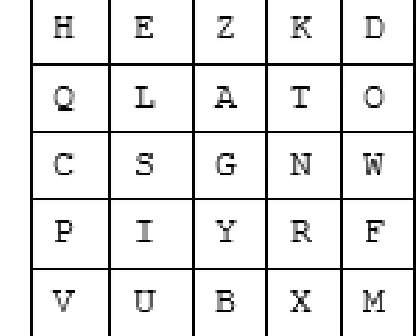
\includegraphics[width=45.57mm,height=92.37mm]{../../images/llm/page_069_img_01.png}%
\end{textblock*}

\end{document}
